\documentclass[12pt,a4paper,oneside]{article}
\usepackage[colorlinks=true,unicode]{hyperref}
\usepackage[utf8]{inputenc}
\usepackage[czech]{babel}
\usepackage{graphicx}
\usepackage{pdfpages}
\textwidth 16cm \textheight 25cm
\topmargin -1.3cm 
\oddsidemargin 0cm
\usepackage{footnote}
\pagestyle{empty}
\begin{document}
\title{Polovodičový releový spínač TRIACSHARP02A}
\author{Jakub Kákona, Miroslav Janás,  kaklik@mlab.cz}
\maketitle

\thispagestyle{empty}
\begin{abstract}
Je určený k experimentálnímu spínání výkonového napájení pro zařízení napájená přímo ze síťového rozvodu jakou jsou například lampy, motory, ventilátory a podobně. Modul má celkem 8 spínaných výstupů.
\end{abstract}

\begin{figure} [htbp]
\begin{center}
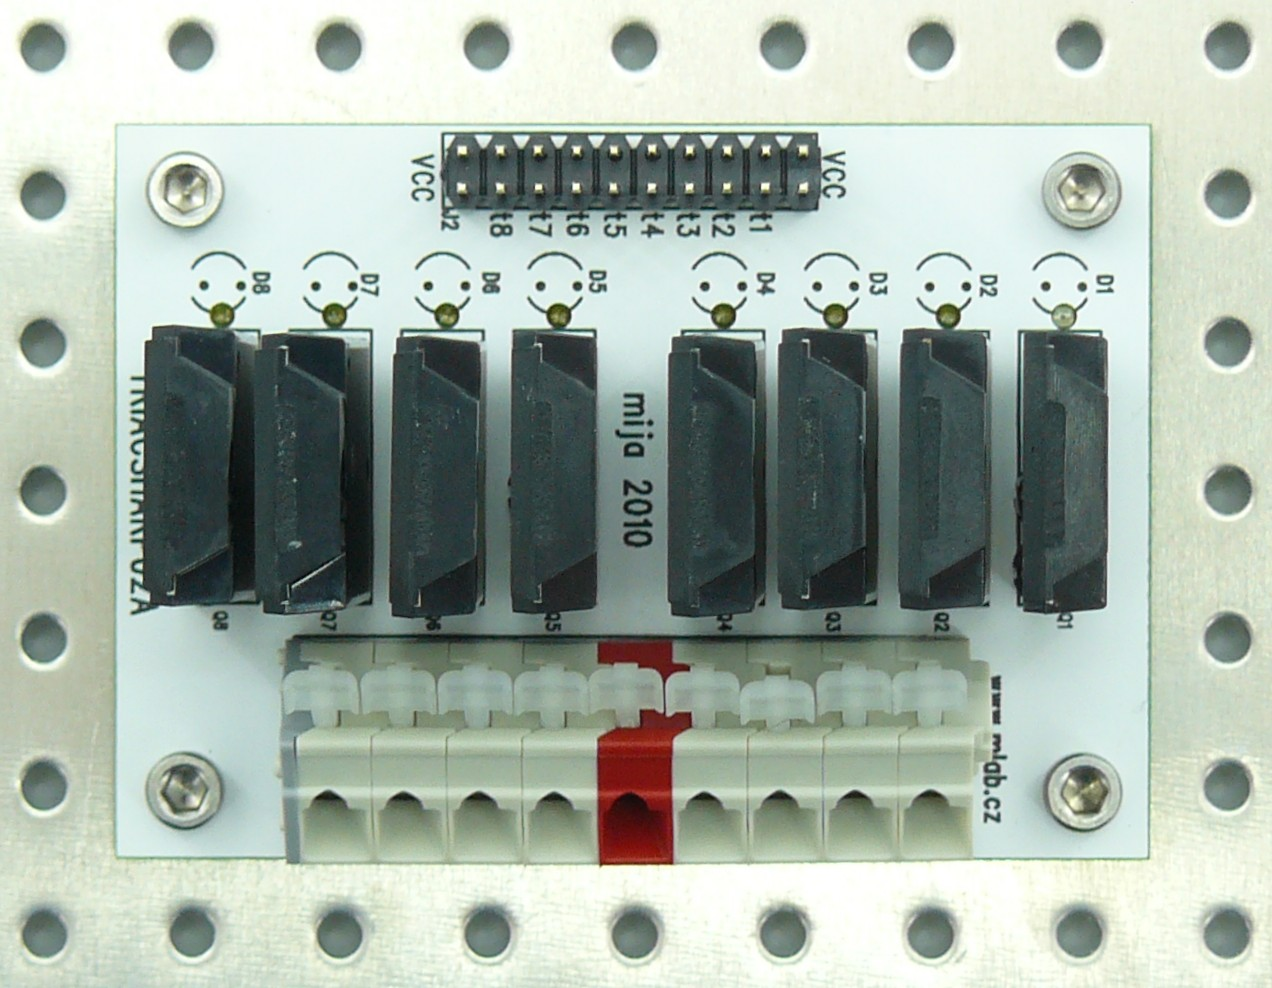
\includegraphics [width=90mm] {./img/TRIACSHARP02A_Top_Big.jpg} 
\end{center}
\end{figure}

\begin{figure} [b]

\includegraphics [width=25mm] {./img/TRIACSHARP02A_QRcode.png} 
\end{figure}

%\newpage
%\tableofcontents


\section{Technické parametry}
\begin{table}[htbp]
\begin{center}
\begin{tabular}{|c|c|c|}
\hline
\multicolumn{1}{|c|}{Parametr} & \multicolumn{1}{|c|}{Hodnota} & \multicolumn{1}{|c|}{Poznámka} \\ \hline
Napájecí napětí Vcc & Typicky +5V &  10mA/kanál \\ \hline
Ovládání kanálů  & Open-emiter & Přizemněním do nuly \\ \hline
Parametry spínání  & max 250V AC @ 8A &  spínání v nule \\ \hline
\end{tabular}
\end{center}
\end{table}

\newpage
\section{Popis konstrukce}

Modul je koncipován, jako spínací prvek pro experimentální zařízení, jako jsou robotické dalekohledy, měřící přístroje, nebo řídící systémy experimentů. 

\subsection{Zapojení}

\begin{figure} [htbp]
%trim option's parameter order: left bottom right top
  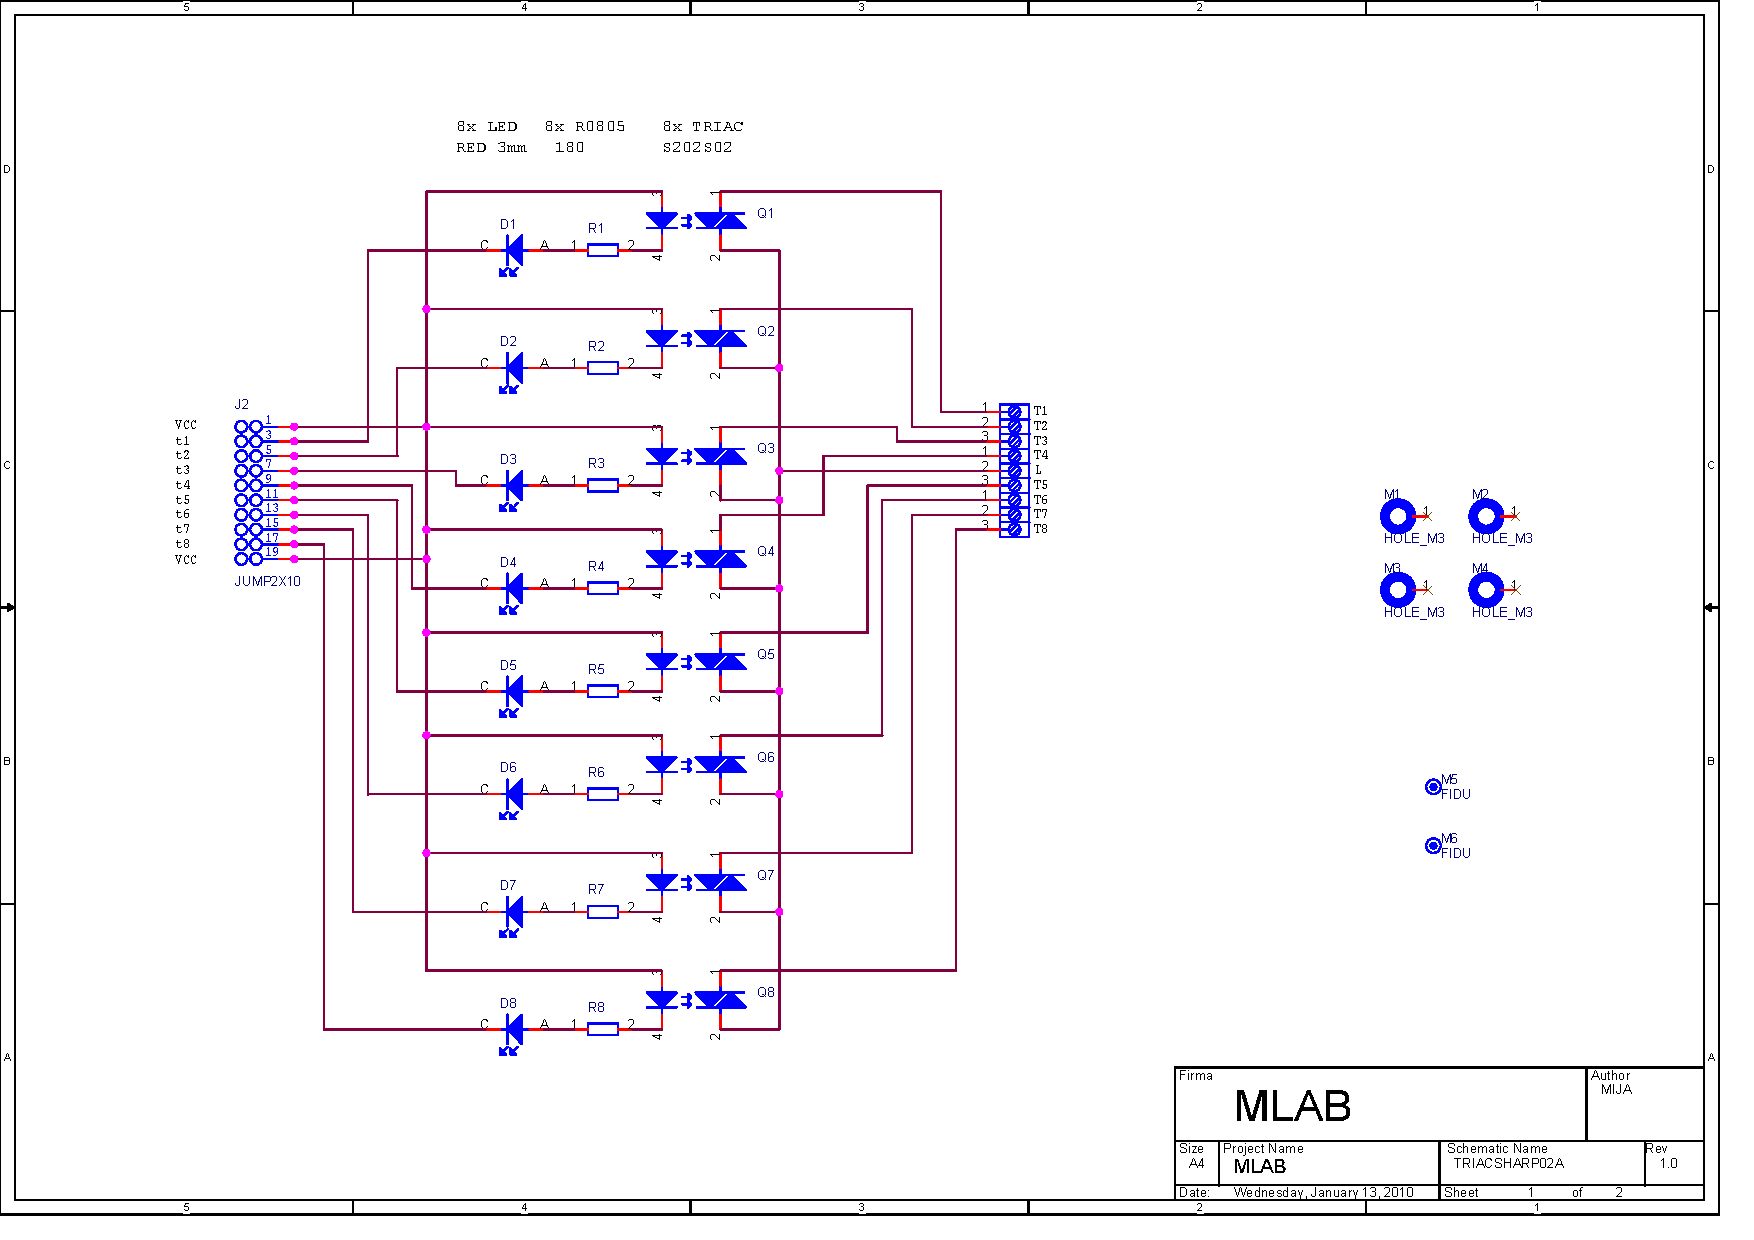
\includegraphics[trim = 5mm 30mm 120mm 15mm, clip, width=15cm]{../../SCH/TRIACSHARP02A.pdf}
\end{figure}

Zapojení modulu předpokládá přivedení fáze na jeden pól svorkovnice označený L na plošném spoji. Polovodičová relé pak spínají tuto fázi na jednotlivé výstupy vyvedené na svorkovnici. Spotřebič se proto k modulu připojuje mezi pracovní nulu (N) a pól svorkovnice. Ochranný vodič PE by měl být připojen k základní desce na které je modul přišroubován. 

\section{Výroba a testování}

\subsection{Osazení}

\begin{figure} [htbp]
%trim option's parameter order: left bottom right top
  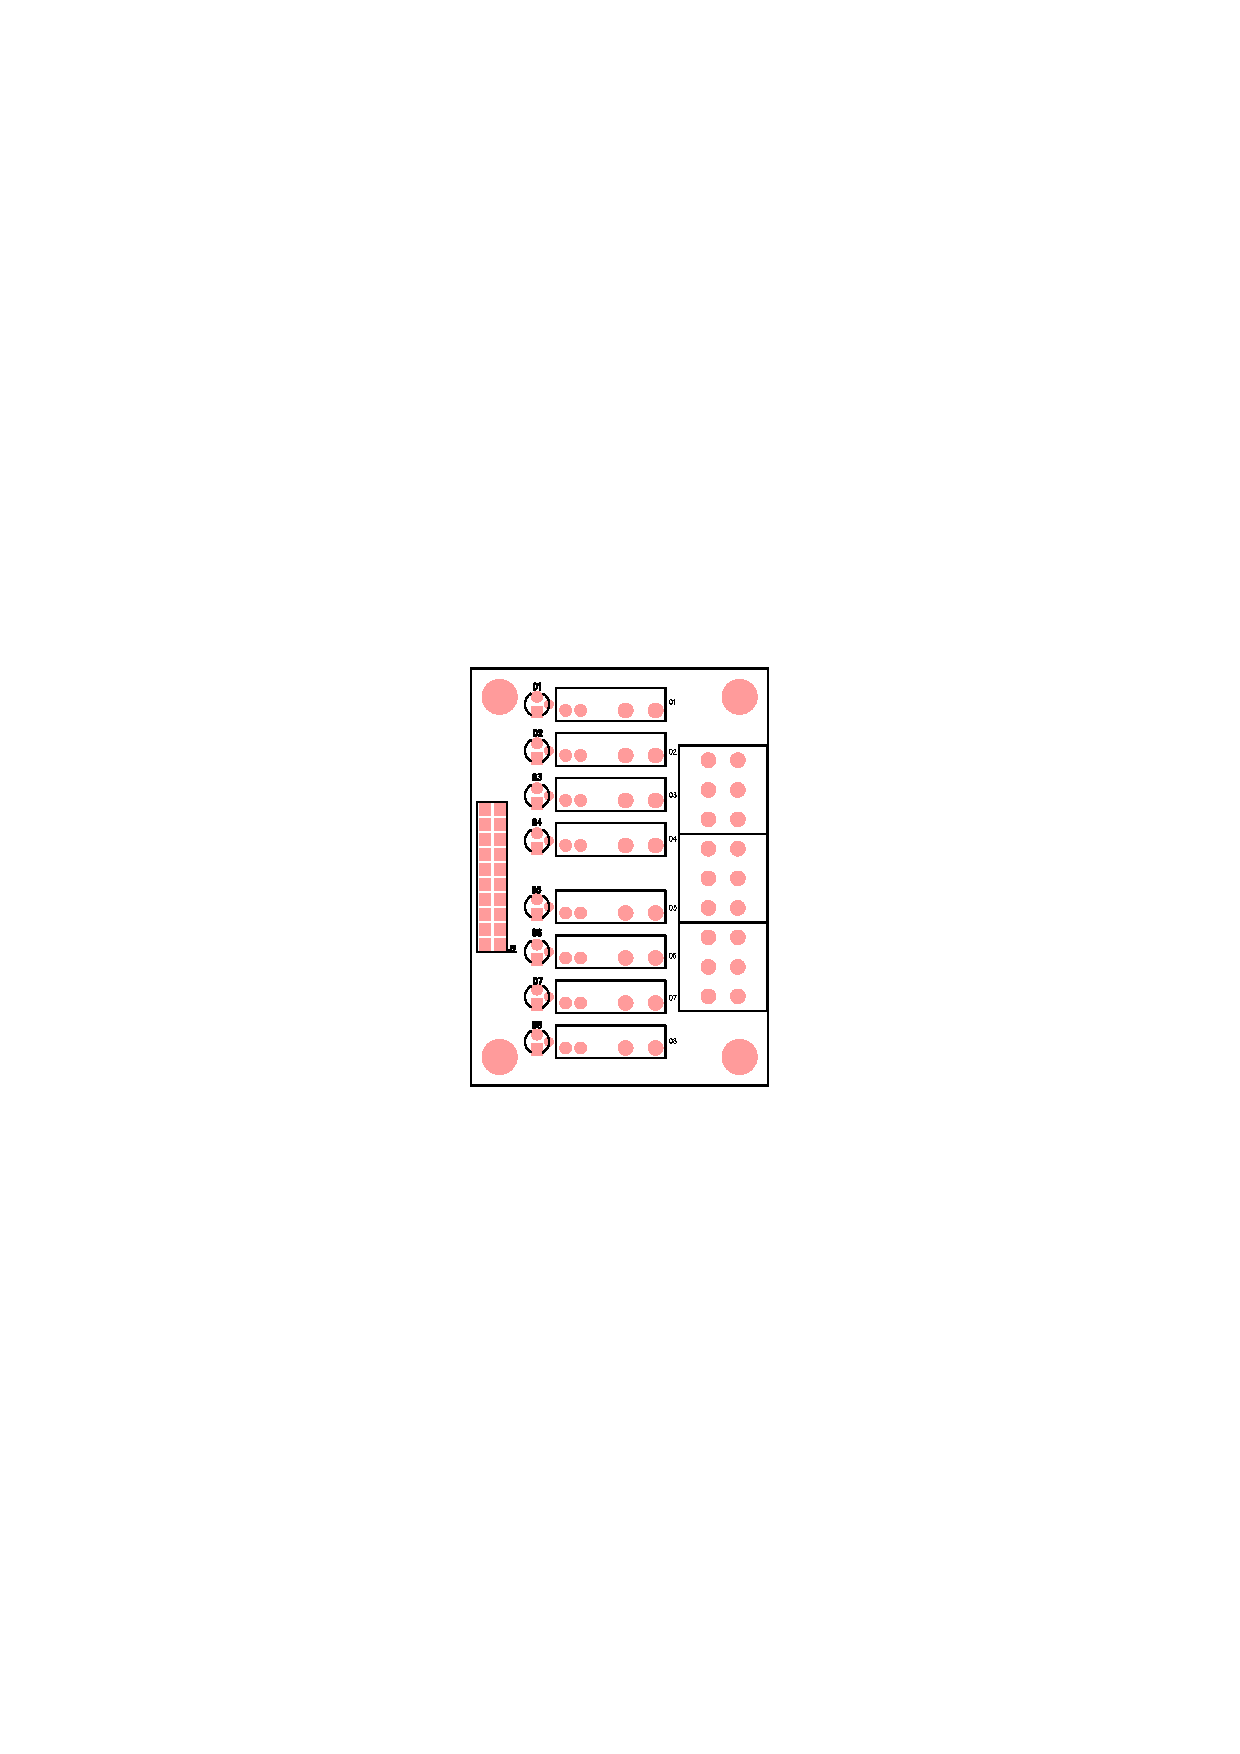
\includegraphics[trim = 70mm 110mm 70mm 110mm, clip, width=8cm]{../../CAM_DOC/O1.pdf}
  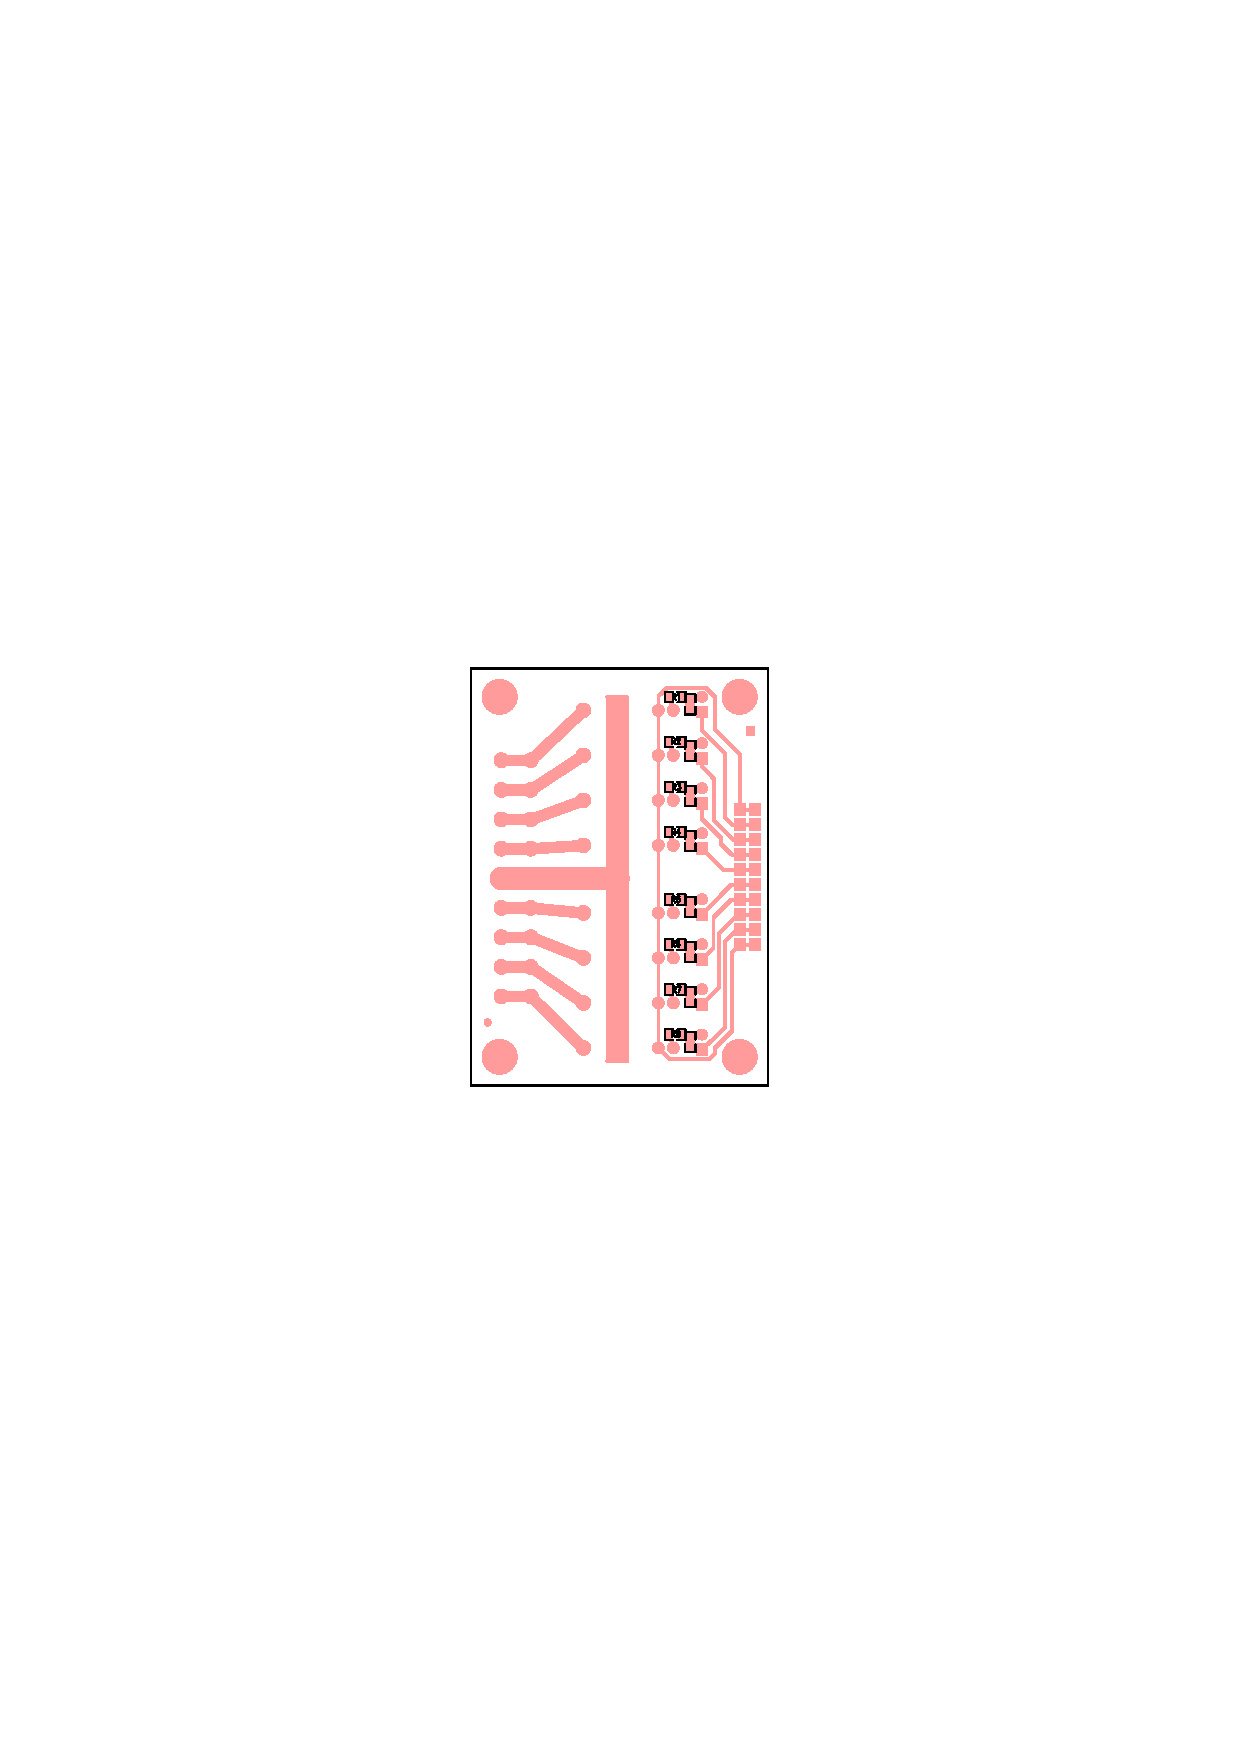
\includegraphics[trim = 70mm 110mm 70mm 110mm, clip, width=8cm]{../../CAM_DOC/O2.pdf}
  \caption{Rozložení součástek na vrchní a spodní straně plošného spoje modulu.}
\end{figure}


\begin{table}
\begin{tabular}{ccc}
Označení & Typ & Pouzdro\\ 
D1,D2,D3,D4,D5,D6,D7,D8	&	LED3		&	RED 3mm \\
J1,J3,J4	 & WAGO 256 & \\ 
J2 &		JUMP2X10		& JUMP2X10 \\
Q1,Q2,Q3,Q4,Q5,Q6,Q7,Q8	& S202S01	&	SIP4 \\
R1,R2,R3,R4,R5,R6,R7,R8 & 180	&  R0805 \\
\end{tabular} 
\end{table}


Na vývody polovodičových relé se během osazování navléká izolační podložka pro LED, která zlepšuje stabilitu a bezpečnost.  Při letování může být přebytečný cín rozlit, po celé ploše odmaskovaných výkonových částí, což zlepšuje výkonové parametry plošného spoje.  Po zaletování všech spojů je modul zespoudu ošetřen bezbarvým vodoodpudivým lakem. 

\begin{figure} [htbp]
\centering
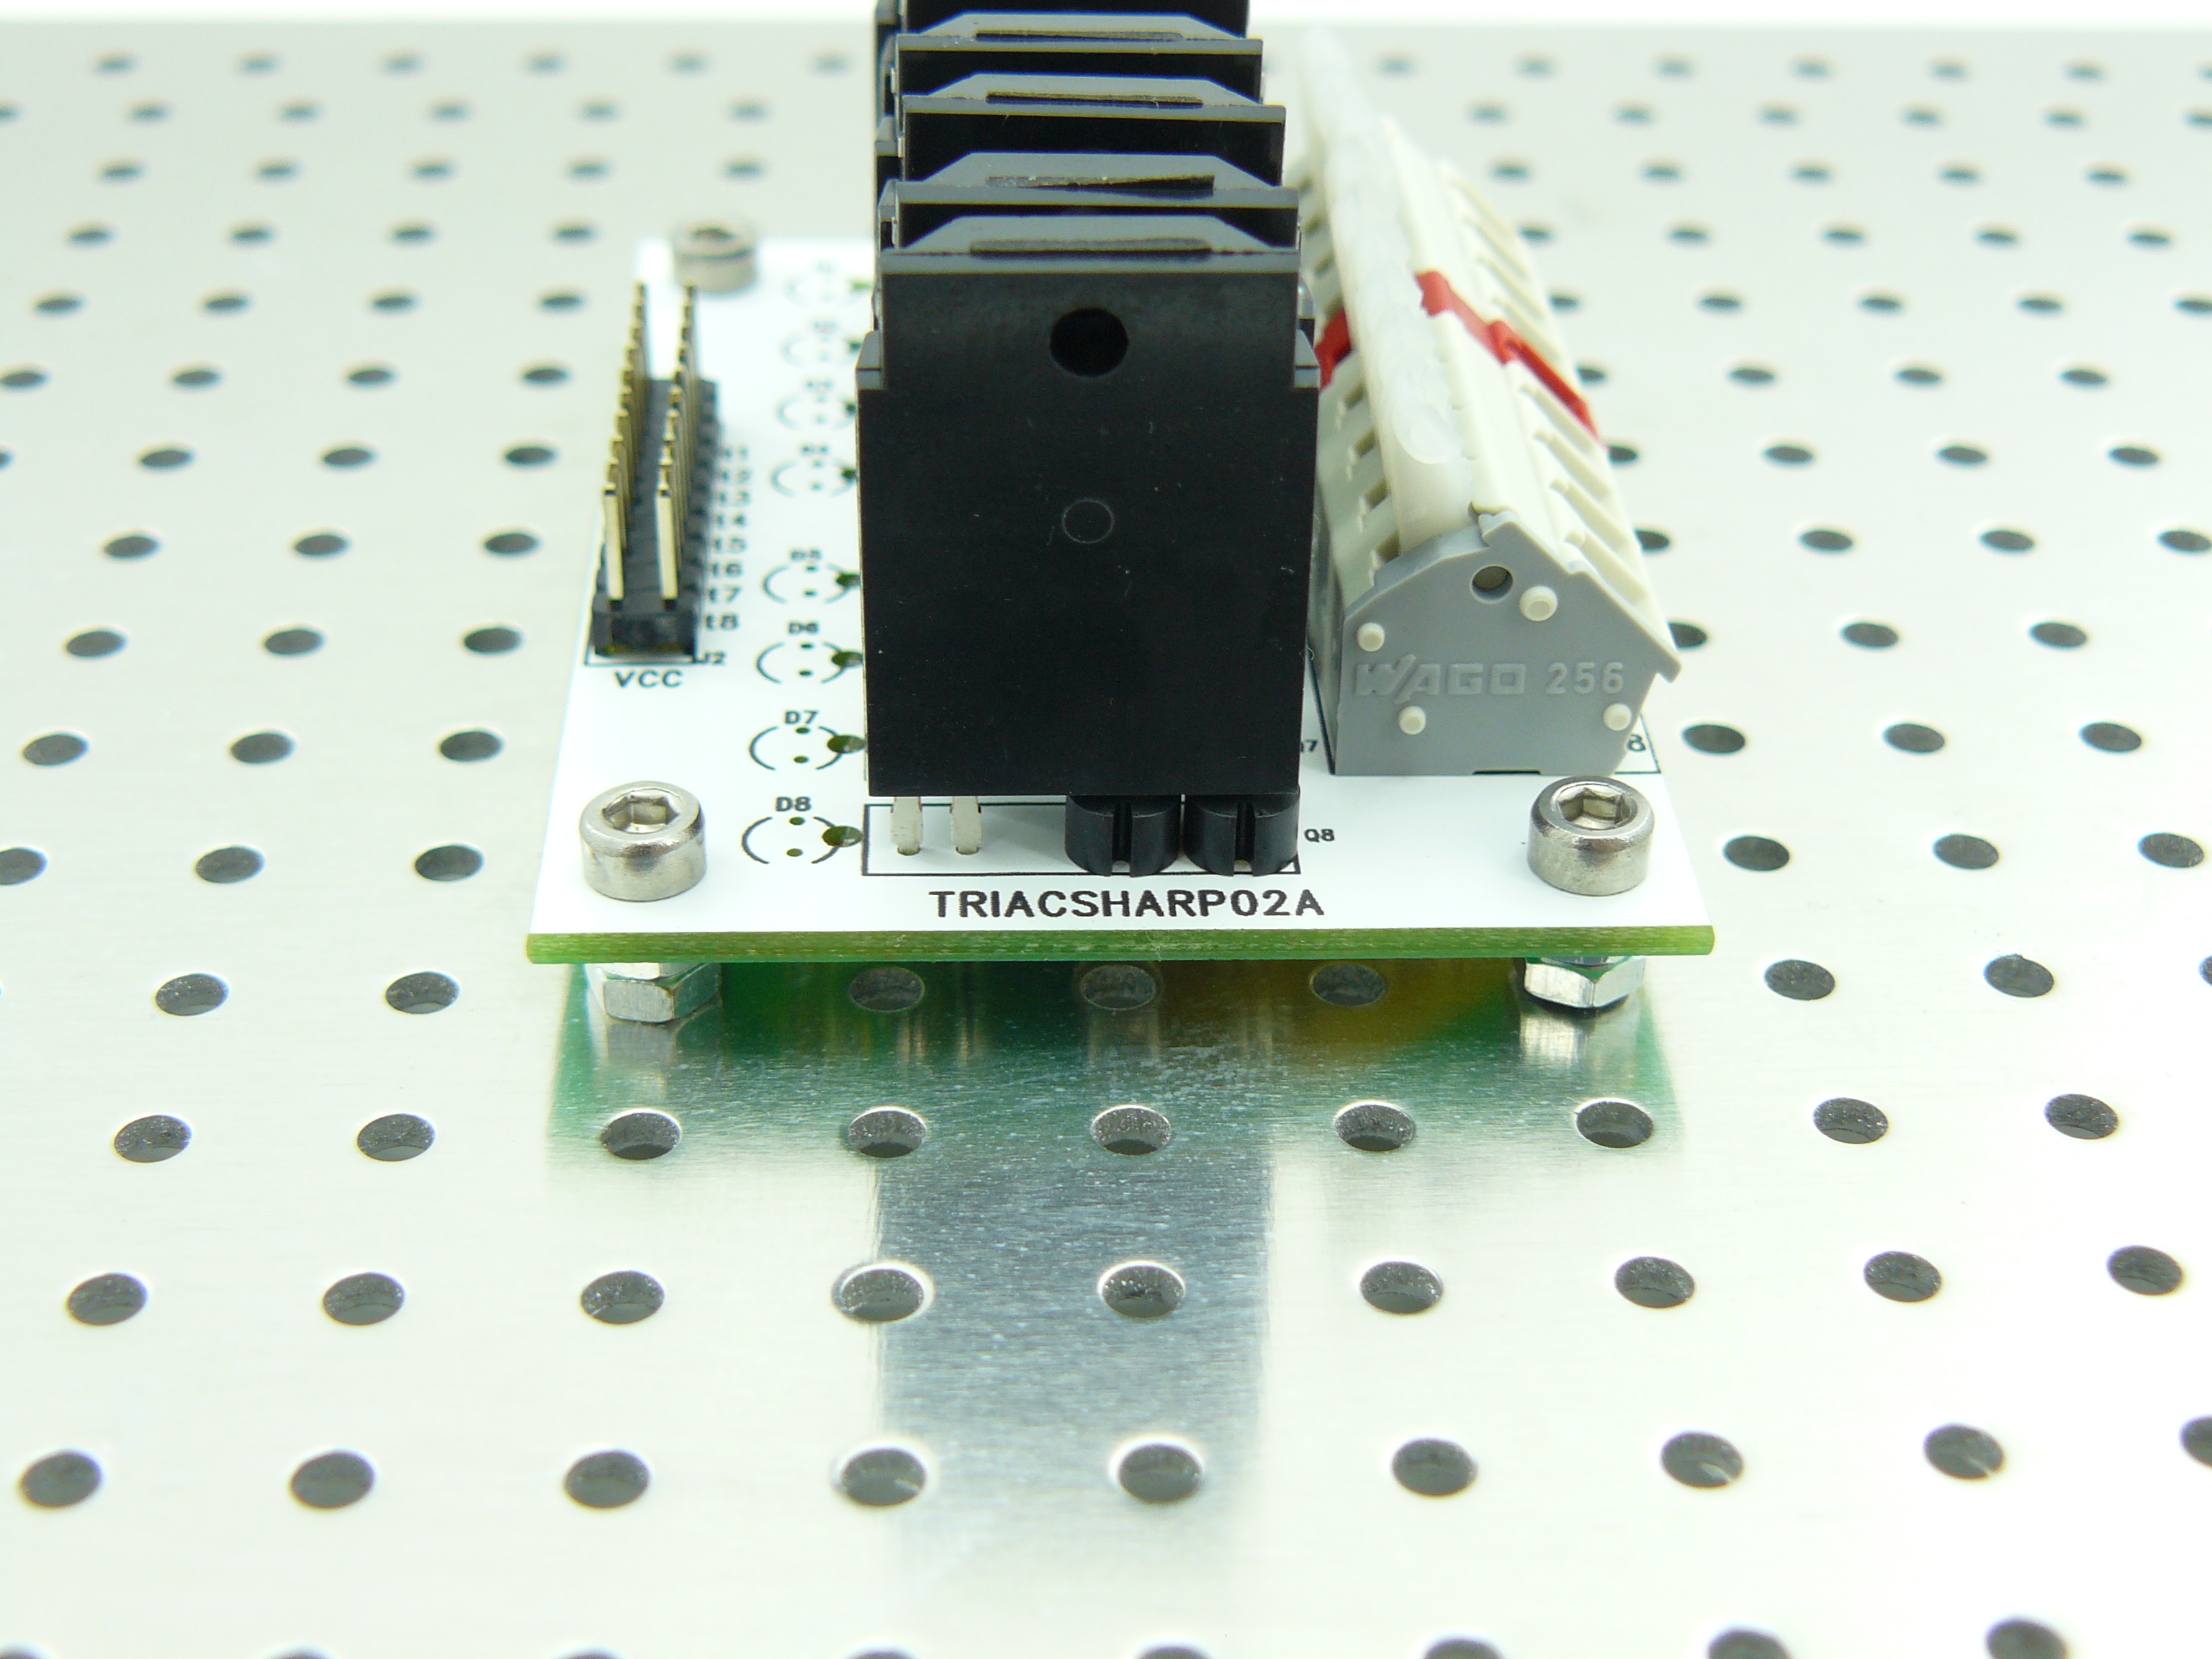
\includegraphics [width=130mm] {./img/TRIACSHARP02A_Big_Side.JPG} 
\end{figure}

\subsection{Ověření funkce}

Modul je testován připojením zásuvky se zapojenou lapičkou s obyčejnou žárovkou. Modul nelze testovat na stejnosměrném napětí, protože triaky, které jsou určeny k spínání střídavého napětí by nerozepnuly.

\section{Použití modulu}

Protože modul dovede spínat i síťové napájecí napětí, tak manipulace s ním může být velmi nebezpečná. S modulem proto mohou manipulovat pouze osoby splňující minimálně požadavky Vyhlášky č. 50/78 Sb., paragrafu 11.

\subsection{Napájení}

Napájecí napětí modulu by mělo odpovídat napájecímu napětí související
logiky. Rezistory zapojené v sérii se spínacími prvky a signalizačními diodami LED jsou v základním osazení dimenzovány pro napájení +5V. Vlivem napěťového úbytku na LED ale není problém na řídící vstupy připojit i logiku 3,3V idální navíc je, pokud bude konstruována, jako open-collector nebo open-drain.

\subsection{Bezpečnost}

Modul má pouze pracovní izolaci. Z hlediska bezpečnosti se s ním proto musí zacházet, jako se zařízením bez izolace. V případě stavebnice MLAB to znamená, že se musí na základní desku šroubovat za použití izolační podložky mezi plošným spojem a základní deskou. Nebo je nutné použít cuprexitovou základní desku otočenou měděnou vrstvou od plošného spoje modulu, tak aby byly zvýšeny izolační parametry zařízení. 

Zároveň výsledné zařízení musí být umístěno v elekroinstalační krabici s krytím a izolací odpovídající požadavkům zvolené aplikace. 

\end{document}